\documentclass[1p]{elsarticle_modified}
%\bibliographystyle{elsarticle-num}

%\usepackage[colorlinks]{hyperref}
%\usepackage{abbrmath_seonhwa} %\Abb, \Ascr, \Acal ,\Abf, \Afrak
\usepackage{amsfonts}
\usepackage{amssymb}
\usepackage{amsmath}
\usepackage{amsthm}
\usepackage{scalefnt}
\usepackage{amsbsy}
\usepackage{kotex}
\usepackage{caption}
\usepackage{subfig}
\usepackage{color}
\usepackage{graphicx}
\usepackage{xcolor} %% white, black, red, green, blue, cyan, magenta, yellow
\usepackage{float}
\usepackage{setspace}
\usepackage{hyperref}

\usepackage{tikz}
\usetikzlibrary{arrows}

\usepackage{multirow}
\usepackage{array} % fixed length table
\usepackage{hhline}

%%%%%%%%%%%%%%%%%%%%%
\makeatletter
\renewcommand*\env@matrix[1][\arraystretch]{%
	\edef\arraystretch{#1}%
	\hskip -\arraycolsep
	\let\@ifnextchar\new@ifnextchar
	\array{*\c@MaxMatrixCols c}}
\makeatother %https://tex.stackexchange.com/questions/14071/how-can-i-increase-the-line-spacing-in-a-matrix
%%%%%%%%%%%%%%%

\usepackage[normalem]{ulem}

\newcommand{\msout}[1]{\ifmmode\text{\sout{\ensuremath{#1}}}\else\sout{#1}\fi}
%SOURCE: \msout is \stkout macro in https://tex.stackexchange.com/questions/20609/strikeout-in-math-mode

\newcommand{\cancel}[1]{
	\ifmmode
	{\color{red}\msout{#1}}
	\else
	{\color{red}\sout{#1}}
	\fi
}

\newcommand{\add}[1]{
	{\color{blue}\uwave{#1}}
}

\newcommand{\replace}[2]{
	\ifmmode
	{\color{red}\msout{#1}}{\color{blue}\uwave{#2}}
	\else
	{\color{red}\sout{#1}}{\color{blue}\uwave{#2}}
	\fi
}

\newcommand{\Sol}{\mathcal{S}} %segment
\newcommand{\D}{D} %diagram
\newcommand{\A}{\mathcal{A}} %arc


%%%%%%%%%%%%%%%%%%%%%%%%%%%%%5 test

\def\sl{\operatorname{\textup{SL}}(2,\Cbb)}
\def\psl{\operatorname{\textup{PSL}}(2,\Cbb)}
\def\quan{\mkern 1mu \triangleright \mkern 1mu}

\theoremstyle{definition}
\newtheorem{thm}{Theorem}[section]
\newtheorem{prop}[thm]{Proposition}
\newtheorem{lem}[thm]{Lemma}
\newtheorem{ques}[thm]{Question}
\newtheorem{cor}[thm]{Corollary}
\newtheorem{defn}[thm]{Definition}
\newtheorem{exam}[thm]{Example}
\newtheorem{rmk}[thm]{Remark}
\newtheorem{alg}[thm]{Algorithm}

\newcommand{\I}{\sqrt{-1}}
\begin{document}

%\begin{frontmatter}
%
%\title{Boundary parabolic representations of knots up to 8 crossings}
%
%%% Group authors per affiliation:
%\author{Yunhi Cho} 
%\address{Department of Mathematics, University of Seoul, Seoul, Korea}
%\ead{yhcho@uos.ac.kr}
%
%
%\author{Seonhwa Kim} %\fnref{s_kim}}
%\address{Center for Geometry and Physics, Institute for Basic Science, Pohang, 37673, Korea}
%\ead{ryeona17@ibs.re.kr}
%
%\author{Hyuk Kim}
%\address{Department of Mathematical Sciences, Seoul National University, Seoul 08826, Korea}
%\ead{hyukkim@snu.ac.kr}
%
%\author{Seokbeom Yoon}
%\address{Department of Mathematical Sciences, Seoul National University, Seoul, 08826,  Korea}
%\ead{sbyoon15@snu.ac.kr}
%
%\begin{abstract}
%We find all boundary parabolic representation of knots up to 8 crossings.
%
%\end{abstract}
%\begin{keyword}
%    \MSC[2010] 57M25 
%\end{keyword}
%
%\end{frontmatter}

%\linenumbers
%\tableofcontents
%
\newcommand\colored[1]{\textcolor{white}{\rule[-0.35ex]{0.8em}{1.4ex}}\kern-0.8em\color{red} #1}%
%\newcommand\colored[1]{\textcolor{white}{ #1}\kern-2.17ex	\textcolor{white}{ #1}\kern-1.81ex	\textcolor{white}{ #1}\kern-2.15ex\color{red}#1	}

{\Large $\underline{12n_{0486}~(K12n_{0486})}$}

\setlength{\tabcolsep}{10pt}
\renewcommand{\arraystretch}{1.6}
\vspace{1cm}\begin{tabular}{m{100pt}>{\centering\arraybackslash}m{274pt}}
\multirow{5}{120pt}{
	\centering
	\includegraphics[width=112pt]{../../../GIT/diagram.site/Diagrams/png/2575_12n_0486.png}\\
\ \ \ A knot diagram\footnotemark}&
\allowdisplaybreaks
\textbf{Linearized knot diagam} \\
\cline{2-2}
 &
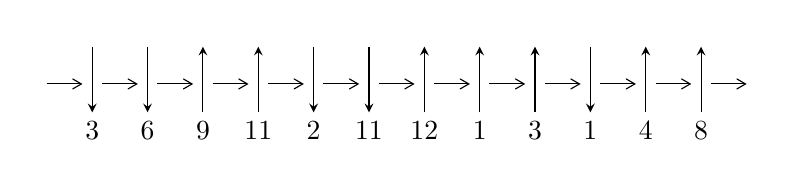
\begin{tikzpicture}[x=20pt, y=17pt]
	% nodes
	\node (C0) at (0, 0) {};
	\node (C1) at (1, 0) {};
	\node (C1U) at (1, +1) {};
	\node (C1D) at (1, -1) {3};

	\node (C2) at (2, 0) {};
	\node (C2U) at (2, +1) {};
	\node (C2D) at (2, -1) {6};

	\node (C3) at (3, 0) {};
	\node (C3U) at (3, +1) {};
	\node (C3D) at (3, -1) {9};

	\node (C4) at (4, 0) {};
	\node (C4U) at (4, +1) {};
	\node (C4D) at (4, -1) {11};

	\node (C5) at (5, 0) {};
	\node (C5U) at (5, +1) {};
	\node (C5D) at (5, -1) {2};

	\node (C6) at (6, 0) {};
	\node (C6U) at (6, +1) {};
	\node (C6D) at (6, -1) {11};

	\node (C7) at (7, 0) {};
	\node (C7U) at (7, +1) {};
	\node (C7D) at (7, -1) {12};

	\node (C8) at (8, 0) {};
	\node (C8U) at (8, +1) {};
	\node (C8D) at (8, -1) {1};

	\node (C9) at (9, 0) {};
	\node (C9U) at (9, +1) {};
	\node (C9D) at (9, -1) {3};

	\node (C10) at (10, 0) {};
	\node (C10U) at (10, +1) {};
	\node (C10D) at (10, -1) {1};

	\node (C11) at (11, 0) {};
	\node (C11U) at (11, +1) {};
	\node (C11D) at (11, -1) {4};

	\node (C12) at (12, 0) {};
	\node (C12U) at (12, +1) {};
	\node (C12D) at (12, -1) {8};
	\node (C13) at (13, 0) {};

	% arrows
	\draw[->,>={angle 60}]
	(C0) edge (C1) (C1) edge (C2) (C2) edge (C3) (C3) edge (C4) (C4) edge (C5) (C5) edge (C6) (C6) edge (C7) (C7) edge (C8) (C8) edge (C9) (C9) edge (C10) (C10) edge (C11) (C11) edge (C12) (C12) edge (C13) ;	\draw[->,>=stealth]
	(C1U) edge (C1D) (C2U) edge (C2D) (C3D) edge (C3U) (C4D) edge (C4U) (C5U) edge (C5D) (C6U) edge (C6D) (C7D) edge (C7U) (C8D) edge (C8U) (C9D) edge (C9U) (C10U) edge (C10D) (C11D) edge (C11U) (C12D) edge (C12U) ;
	\end{tikzpicture} \\
\hhline{~~} \\& 
\textbf{Solving Sequence} \\ \cline{2-2} 
 &
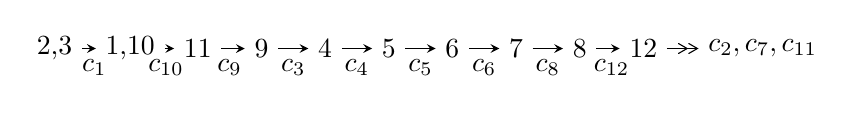
\begin{tikzpicture}[x=23pt, y=7pt]
	% node
	\node (A0) at (-1/8, 0) {2,3};
	\node (A1) at (17/16, 0) {1,10};
	\node (A2) at (17/8, 0) {11};
	\node (A3) at (25/8, 0) {9};
	\node (A4) at (33/8, 0) {4};
	\node (A5) at (41/8, 0) {5};
	\node (A6) at (49/8, 0) {6};
	\node (A7) at (57/8, 0) {7};
	\node (A8) at (65/8, 0) {8};
	\node (A9) at (73/8, 0) {12};
	\node (C1) at (1/2, -1) {$c_{1}$};
	\node (C2) at (13/8, -1) {$c_{10}$};
	\node (C3) at (21/8, -1) {$c_{9}$};
	\node (C4) at (29/8, -1) {$c_{3}$};
	\node (C5) at (37/8, -1) {$c_{4}$};
	\node (C6) at (45/8, -1) {$c_{5}$};
	\node (C7) at (53/8, -1) {$c_{6}$};
	\node (C8) at (61/8, -1) {$c_{8}$};
	\node (C9) at (69/8, -1) {$c_{12}$};
	\node (A10) at (11, 0) {$c_{2},c_{7},c_{11}$};

	% edge
	\draw[->,>=stealth]	
	(A0) edge (A1) (A1) edge (A2) (A2) edge (A3) (A3) edge (A4) (A4) edge (A5) (A5) edge (A6) (A6) edge (A7) (A7) edge (A8) (A8) edge (A9) ;
	\draw[->>,>={angle 60}]	
	(A9) edge (A10);
\end{tikzpicture} \\ 

\end{tabular} \\

\footnotetext{
The image of knot diagram is generated by the software ``\textbf{Draw programme}" developed by Andrew Bartholomew(\url{http://www.layer8.co.uk/maths/draw/index.htm\#Running-draw}), where we modified some parts for our purpose(\url{https://github.com/CATsTAILs/LinksPainter}).
}\phantom \\ \newline 
\centering \textbf{Ideals for irreducible components\footnotemark of $X_{\text{par}}$} 
 
\begin{align*}
I^u_{1}&=\langle 
-29739878226279 u^{18}+120434793497659 u^{17}+\cdots+532958163092980 b-59832203175112,\\
\phantom{I^u_{1}}&\phantom{= \langle  }-9362493576748 u^{18}+40768461372003 u^{17}+\cdots+532958163092980 a-81214256524619,\\
\phantom{I^u_{1}}&\phantom{= \langle  }u^{19}-5 u^{18}+\cdots+12 u-16\rangle \\
I^u_{2}&=\langle 
- u^{10}+4 u^9-13 u^8+29 u^7-51 u^6+74 u^5-84 u^4+78 u^3-54 u^2+b+26 u-6,\\
\phantom{I^u_{2}}&\phantom{= \langle  }-3 u^{11}+12 u^{10}-41 u^9+96 u^8-179 u^7+277 u^6-338 u^5+345 u^4-274 u^3+163 u^2+a-67 u+13,\\
\phantom{I^u_{2}}&\phantom{= \langle  }u^{12}-4 u^{11}+14 u^{10}-33 u^9+63 u^8-99 u^7+124 u^6-131 u^5+108 u^4-70 u^3+32 u^2-9 u+1\rangle \\
I^u_{3}&=\langle 
2 u^4 a^3-11 u^4 a^2+\cdots+2 a-17,\;3 u^4 a^2+9 u^4 a+\cdots+19 a-25,\;u^5- u^4+4 u^3-3 u^2+3 u-1\rangle \\
\\
\end{align*}
\raggedright * 3 irreducible components of $\dim_{\mathbb{C}}=0$, with total 51 representations.\\
\footnotetext{All coefficients of polynomials are rational numbers. But the coefficients are sometimes approximated in decimal forms when there is not enough margin.}
\newpage
\renewcommand{\arraystretch}{1}
\centering \section*{I. $I^u_{1}= \langle -2.97\times10^{13} u^{18}+1.20\times10^{14} u^{17}+\cdots+5.33\times10^{14} b-5.98\times10^{13},\;-9.36\times10^{12} u^{18}+4.08\times10^{13} u^{17}+\cdots+5.33\times10^{14} a-8.12\times10^{13},\;u^{19}-5 u^{18}+\cdots+12 u-16 \rangle$}
\flushleft \textbf{(i) Arc colorings}\\
\begin{tabular}{m{7pt} m{180pt} m{7pt} m{180pt} }
\flushright $a_{2}=$&$\begin{pmatrix}1\\0\end{pmatrix}$ \\
\flushright $a_{3}=$&$\begin{pmatrix}0\\u\end{pmatrix}$ \\
\flushright $a_{1}=$&$\begin{pmatrix}1\\- u^2\end{pmatrix}$ \\
\flushright $a_{10}=$&$\begin{pmatrix}0.0175670 u^{18}-0.0764947 u^{17}+\cdots+4.43978 u+0.152384\\0.0558015 u^{18}-0.225974 u^{17}+\cdots+0.918202 u+0.112264\end{pmatrix}$ \\
\flushright $a_{11}=$&$\begin{pmatrix}-0.00459523 u^{18}+0.0200061 u^{17}+\cdots+3.37659 u-0.141328\\0.00804171 u^{18}-0.0413187 u^{17}+\cdots+1.10107 u+0.341233\end{pmatrix}$ \\
\flushright $a_{9}=$&$\begin{pmatrix}0.0175670 u^{18}-0.0764947 u^{17}+\cdots+4.43978 u+0.152384\\0.0221623 u^{18}-0.0965008 u^{17}+\cdots+1.06319 u+0.293712\end{pmatrix}$ \\
\flushright $a_{4}=$&$\begin{pmatrix}0.0168589 u^{18}-0.0901711 u^{17}+\cdots-2.65099 u+0.926294\\0.0247508 u^{18}-0.110253 u^{17}+\cdots-0.106730 u+0.303577\end{pmatrix}$ \\
\flushright $a_{5}=$&$\begin{pmatrix}0.00896711 u^{18}-0.0700889 u^{17}+\cdots-4.19525 u+1.54901\\0.0662912 u^{18}-0.290418 u^{17}+\cdots-1.31972 u+0.917186\end{pmatrix}$ \\
\flushright $a_{6}=$&$\begin{pmatrix}-0.0573241 u^{18}+0.220329 u^{17}+\cdots-2.87554 u+0.631826\\0.0662912 u^{18}-0.290418 u^{17}+\cdots-1.31972 u+0.917186\end{pmatrix}$ \\
\flushright $a_{7}=$&$\begin{pmatrix}-0.0618479 u^{18}+0.231160 u^{17}+\cdots-1.58362 u+0.249407\\0.0729756 u^{18}-0.306781 u^{17}+\cdots-0.884238 u+0.609177\end{pmatrix}$ \\
\flushright $a_{8}=$&$\begin{pmatrix}0.0290440 u^{18}-0.109467 u^{17}+\cdots+3.23161 u-0.322776\\-0.0303669 u^{18}+0.123682 u^{17}+\cdots+1.17250 u-0.0968854\end{pmatrix}$ \\
\flushright $a_{12}=$&$\begin{pmatrix}-0.0146657 u^{18}+0.0593565 u^{17}+\cdots+1.94146 u+0.302400\\0.0190316 u^{18}-0.0849051 u^{17}+\cdots+0.645986 u+0.311849\end{pmatrix}$\\&\end{tabular}
\flushleft \textbf{(ii) Obstruction class $= -1$}\\~\\
\flushleft \textbf{(iii) Cusp Shapes $= -\frac{51647443263187}{133239540773245} u^{18}+\frac{248046807631858}{133239540773245} u^{17}+\cdots-\frac{45855187936601}{7837620045485} u-\frac{9980369352966}{26647908154649}$}\\~\\
\newpage\renewcommand{\arraystretch}{1}
\flushleft \textbf{(iv) u-Polynomials at the component}\newline \\
\begin{tabular}{m{50pt}|m{274pt}}
Crossings & \hspace{64pt}u-Polynomials at each crossing \\
\hline $$\begin{aligned}c_{1}\end{aligned}$$&$\begin{aligned}
&u^{19}+5 u^{18}+\cdots+12 u+16
\end{aligned}$\\
\hline $$\begin{aligned}c_{2},c_{5}\end{aligned}$$&$\begin{aligned}
&u^{19}+5 u^{18}+\cdots+6 u+4
\end{aligned}$\\
\hline $$\begin{aligned}c_{3},c_{4},c_{9}\\c_{11}\end{aligned}$$&$\begin{aligned}
&u^{19}-4 u^{17}+\cdots+u-1
\end{aligned}$\\
\hline $$\begin{aligned}c_{6},c_{10}\end{aligned}$$&$\begin{aligned}
&u^{19}-2 u^{18}+\cdots+17 u+1
\end{aligned}$\\
\hline $$\begin{aligned}c_{7},c_{8},c_{12}\end{aligned}$$&$\begin{aligned}
&u^{19}+9 u^{18}+\cdots+96 u+32
\end{aligned}$\\
\hline
\end{tabular}\\~\\
\newpage\renewcommand{\arraystretch}{1}
\flushleft \textbf{(v) Riley Polynomials at the component}\newline \\
\begin{tabular}{m{50pt}|m{274pt}}
Crossings & \hspace{64pt}Riley Polynomials at each crossing \\
\hline $$\begin{aligned}c_{1}\end{aligned}$$&$\begin{aligned}
&y^{19}+19 y^{18}+\cdots-2960 y-256
\end{aligned}$\\
\hline $$\begin{aligned}c_{2},c_{5}\end{aligned}$$&$\begin{aligned}
&y^{19}-5 y^{18}+\cdots+12 y-16
\end{aligned}$\\
\hline $$\begin{aligned}c_{3},c_{4},c_{9}\\c_{11}\end{aligned}$$&$\begin{aligned}
&y^{19}-8 y^{18}+\cdots+3 y-1
\end{aligned}$\\
\hline $$\begin{aligned}c_{6},c_{10}\end{aligned}$$&$\begin{aligned}
&y^{19}+48 y^{18}+\cdots+103 y-1
\end{aligned}$\\
\hline $$\begin{aligned}c_{7},c_{8},c_{12}\end{aligned}$$&$\begin{aligned}
&y^{19}-19 y^{18}+\cdots+1536 y-1024
\end{aligned}$\\
\hline
\end{tabular}\\~\\
\newpage\flushleft \textbf{(vi) Complex Volumes and Cusp Shapes}
$$\begin{array}{c|c|c}  
\text{Solutions to }I^u_{1}& \I (\text{vol} + \sqrt{-1}CS) & \text{Cusp shape}\\
 \hline 
\begin{aligned}
u &= \phantom{-}0.722196 + 0.657529 I \\
a &= \phantom{-}0.102214 - 0.799363 I \\
b &= -1.17960 - 0.94405 I\end{aligned}
 & -0.82235 - 3.78512 I & \phantom{-}1.21860 + 9.00060 I \\ \hline\begin{aligned}
u &= \phantom{-}0.722196 - 0.657529 I \\
a &= \phantom{-}0.102214 + 0.799363 I \\
b &= -1.17960 + 0.94405 I\end{aligned}
 & -0.82235 + 3.78512 I & \phantom{-}1.21860 - 9.00060 I \\ \hline\begin{aligned}
u &= -0.746643 + 0.730089 I \\
a &= -0.462703 - 1.042820 I \\
b &= \phantom{-}0.810875 - 1.125140 I\end{aligned}
 & \phantom{-}7.60259 + 2.70738 I & \phantom{-}8.67277 - 2.95502 I \\ \hline\begin{aligned}
u &= -0.746643 - 0.730089 I \\
a &= -0.462703 + 1.042820 I \\
b &= \phantom{-}0.810875 + 1.125140 I\end{aligned}
 & \phantom{-}7.60259 - 2.70738 I & \phantom{-}8.67277 + 2.95502 I \\ \hline\begin{aligned}
u &= \phantom{-}0.693820 + 0.494332 I \\
a &= \phantom{-}0.456624 + 0.344671 I \\
b &= -0.060397 - 0.381407 I\end{aligned}
 & -1.48005 - 1.04351 I & -2.45665 + 0.14135 I \\ \hline\begin{aligned}
u &= \phantom{-}0.693820 - 0.494332 I \\
a &= \phantom{-}0.456624 - 0.344671 I \\
b &= -0.060397 + 0.381407 I\end{aligned}
 & -1.48005 + 1.04351 I & -2.45665 - 0.14135 I \\ \hline\begin{aligned}
u &= -0.04060 + 1.46804 I \\
a &= -0.307074 + 0.628614 I \\
b &= -0.45900 + 3.71191 I\end{aligned}
 & \phantom{-}6.95938 + 1.17078 I & \phantom{-}6.09940 - 4.23132 I \\ \hline\begin{aligned}
u &= -0.04060 - 1.46804 I \\
a &= -0.307074 - 0.628614 I \\
b &= -0.45900 - 3.71191 I\end{aligned}
 & \phantom{-}6.95938 - 1.17078 I & \phantom{-}6.09940 + 4.23132 I \\ \hline\begin{aligned}
u &= \phantom{-}0.89865 + 1.22513 I \\
a &= \phantom{-}0.029251 + 0.797483 I \\
b &= \phantom{-}2.06454 + 1.29373 I\end{aligned}
 & \phantom{-}5.18478 - 8.09242 I & \phantom{-}3.53036 + 7.90230 I \\ \hline\begin{aligned}
u &= \phantom{-}0.89865 - 1.22513 I \\
a &= \phantom{-}0.029251 - 0.797483 I \\
b &= \phantom{-}2.06454 - 1.29373 I\end{aligned}
 & \phantom{-}5.18478 + 8.09242 I & \phantom{-}3.53036 - 7.90230 I\\
 \hline 
 \end{array}$$\newpage$$\begin{array}{c|c|c}  
\text{Solutions to }I^u_{1}& \I (\text{vol} + \sqrt{-1}CS) & \text{Cusp shape}\\
 \hline 
\begin{aligned}
u &= \phantom{-}0.24994 + 1.58443 I \\
a &= -0.240884 - 0.605481 I \\
b &= -1.19770 - 3.77858 I\end{aligned}
 & \phantom{-}6.58876 - 7.45308 I & \phantom{-}5.69466 + 9.39888 I \\ \hline\begin{aligned}
u &= \phantom{-}0.24994 - 1.58443 I \\
a &= -0.240884 + 0.605481 I \\
b &= -1.19770 + 3.77858 I\end{aligned}
 & \phantom{-}6.58876 + 7.45308 I & \phantom{-}5.69466 - 9.39888 I \\ \hline\begin{aligned}
u &= \phantom{-}1.63895\phantom{ +0.000000I} \\
a &= -0.425083\phantom{ +0.000000I} \\
b &= \phantom{-}1.00806\phantom{ +0.000000I}\end{aligned}
 & \phantom{-}1.14876\phantom{ +0.000000I} & \phantom{-}15.5300\phantom{ +0.000000I} \\ \hline\begin{aligned}
u &= -0.158529 + 0.292224 I \\
a &= \phantom{-}0.28403 + 1.88623 I \\
b &= \phantom{-}0.221614 + 0.650228 I\end{aligned}
 & \phantom{-}1.090730 + 0.511038 I & \phantom{-}7.83780 - 2.24263 I \\ \hline\begin{aligned}
u &= -0.158529 - 0.292224 I \\
a &= \phantom{-}0.28403 - 1.88623 I \\
b &= \phantom{-}0.221614 - 0.650228 I\end{aligned}
 & \phantom{-}1.090730 - 0.511038 I & \phantom{-}7.83780 + 2.24263 I \\ \hline\begin{aligned}
u &= -0.20388 + 1.65874 I \\
a &= \phantom{-}0.557769 - 0.904546 I \\
b &= \phantom{-}2.54312 - 4.44242 I\end{aligned}
 & \phantom{-}15.7917 + 6.1961 I & \phantom{-}6.23161 - 1.95293 I \\ \hline\begin{aligned}
u &= -0.20388 - 1.65874 I \\
a &= \phantom{-}0.557769 + 0.904546 I \\
b &= \phantom{-}2.54312 + 4.44242 I\end{aligned}
 & \phantom{-}15.7917 - 6.1961 I & \phantom{-}6.23161 + 1.95293 I \\ \hline\begin{aligned}
u &= \phantom{-}0.26558 + 1.78867 I \\
a &= \phantom{-}0.543309 + 0.825825 I \\
b &= \phantom{-}3.25252 + 4.45796 I\end{aligned}
 & \phantom{-}15.2603 - 12.9682 I & \phantom{-}5.40622 + 6.37379 I \\ \hline\begin{aligned}
u &= \phantom{-}0.26558 - 1.78867 I \\
a &= \phantom{-}0.543309 - 0.825825 I \\
b &= \phantom{-}3.25252 - 4.45796 I\end{aligned}
 & \phantom{-}15.2603 + 12.9682 I & \phantom{-}5.40622 - 6.37379 I\\
 \hline 
 \end{array}$$\newpage\newpage\renewcommand{\arraystretch}{1}
\centering \section*{II. $I^u_{2}= \langle - u^{10}+4 u^9+\cdots+b-6,\;-3 u^{11}+12 u^{10}+\cdots+a+13,\;u^{12}-4 u^{11}+\cdots-9 u+1 \rangle$}
\flushleft \textbf{(i) Arc colorings}\\
\begin{tabular}{m{7pt} m{180pt} m{7pt} m{180pt} }
\flushright $a_{2}=$&$\begin{pmatrix}1\\0\end{pmatrix}$ \\
\flushright $a_{3}=$&$\begin{pmatrix}0\\u\end{pmatrix}$ \\
\flushright $a_{1}=$&$\begin{pmatrix}1\\- u^2\end{pmatrix}$ \\
\flushright $a_{10}=$&$\begin{pmatrix}3 u^{11}-12 u^{10}+\cdots+67 u-13\\u^{10}-4 u^9+\cdots-26 u+6\end{pmatrix}$ \\
\flushright $a_{11}=$&$\begin{pmatrix}4 u^{11}-16 u^{10}+\cdots+96 u-19\\u^{10}-4 u^9+\cdots-25 u+6\end{pmatrix}$ \\
\flushright $a_{9}=$&$\begin{pmatrix}3 u^{11}-12 u^{10}+\cdots+67 u-13\\- u^{11}+4 u^{10}+\cdots-29 u+6\end{pmatrix}$ \\
\flushright $a_{4}=$&$\begin{pmatrix}-5 u^{11}+18 u^{10}+\cdots-78 u+13\\2 u^{11}-7 u^{10}+\cdots+27 u-5\end{pmatrix}$ \\
\flushright $a_{5}=$&$\begin{pmatrix}2 u^{11}-7 u^{10}+\cdots+26 u-5\\- u^{11}+4 u^{10}+\cdots-19 u+3\end{pmatrix}$ \\
\flushright $a_{6}=$&$\begin{pmatrix}3 u^{11}-11 u^{10}+\cdots+45 u-8\\- u^{11}+4 u^{10}+\cdots-19 u+3\end{pmatrix}$ \\
\flushright $a_{7}=$&$\begin{pmatrix}-5 u^{11}+18 u^{10}+\cdots-94 u+21\\3 u^{11}-11 u^{10}+\cdots+48 u-10\end{pmatrix}$ \\
\flushright $a_{8}=$&$\begin{pmatrix}5 u^{11}-19 u^{10}+\cdots+99 u-19\\- u^{11}+5 u^{10}+\cdots-36 u+7\end{pmatrix}$ \\
\flushright $a_{12}=$&$\begin{pmatrix}4 u^{11}-15 u^{10}+\cdots+88 u-20\\-2 u^{11}+7 u^{10}+\cdots-34 u+8\end{pmatrix}$\\&\end{tabular}
\flushleft \textbf{(ii) Obstruction class $= 1$}\\~\\
\flushleft \textbf{(iii) Cusp Shapes $= -13 u^{11}+47 u^{10}-166 u^9+372 u^8-699 u^7+1066 u^6-1282 u^5+1319 u^4-1003 u^3+610 u^2-225 u+43$}\\~\\
\newpage\renewcommand{\arraystretch}{1}
\flushleft \textbf{(iv) u-Polynomials at the component}\newline \\
\begin{tabular}{m{50pt}|m{274pt}}
Crossings & \hspace{64pt}u-Polynomials at each crossing \\
\hline $$\begin{aligned}c_{1}\end{aligned}$$&$\begin{aligned}
&u^{12}-4 u^{11}+\cdots-9 u+1
\end{aligned}$\\
\hline $$\begin{aligned}c_{2}\end{aligned}$$&$\begin{aligned}
&u^{12}-2 u^{10}- u^9+5 u^8+u^7-6 u^6-3 u^5+6 u^4+2 u^3-4 u^2- u+1
\end{aligned}$\\
\hline $$\begin{aligned}c_{3},c_{11}\end{aligned}$$&$\begin{aligned}
&u^{12}+4 u^{10}- u^9+3 u^8-3 u^7-2 u^6- u^5+u^4+u^3+2 u^2- u-1
\end{aligned}$\\
\hline $$\begin{aligned}c_{4},c_{9}\end{aligned}$$&$\begin{aligned}
&u^{12}+4 u^{10}+u^9+3 u^8+3 u^7-2 u^6+u^5+u^4- u^3+2 u^2+u-1
\end{aligned}$\\
\hline $$\begin{aligned}c_{5}\end{aligned}$$&$\begin{aligned}
&u^{12}-2 u^{10}+u^9+5 u^8- u^7-6 u^6+3 u^5+6 u^4-2 u^3-4 u^2+u+1
\end{aligned}$\\
\hline $$\begin{aligned}c_{6},c_{10}\end{aligned}$$&$\begin{aligned}
&u^{12}+4 u^{11}+\cdots+3 u+3
\end{aligned}$\\
\hline $$\begin{aligned}c_{7},c_{8}\end{aligned}$$&$\begin{aligned}
&u^{12}+4 u^{11}+\cdots-3 u+1
\end{aligned}$\\
\hline $$\begin{aligned}c_{12}\end{aligned}$$&$\begin{aligned}
&u^{12}-4 u^{11}+\cdots+3 u+1
\end{aligned}$\\
\hline
\end{tabular}\\~\\
\newpage\renewcommand{\arraystretch}{1}
\flushleft \textbf{(v) Riley Polynomials at the component}\newline \\
\begin{tabular}{m{50pt}|m{274pt}}
Crossings & \hspace{64pt}Riley Polynomials at each crossing \\
\hline $$\begin{aligned}c_{1}\end{aligned}$$&$\begin{aligned}
&y^{12}+12 y^{11}+\cdots-17 y+1
\end{aligned}$\\
\hline $$\begin{aligned}c_{2},c_{5}\end{aligned}$$&$\begin{aligned}
&y^{12}-4 y^{11}+\cdots-9 y+1
\end{aligned}$\\
\hline $$\begin{aligned}c_{3},c_{4},c_{9}\\c_{11}\end{aligned}$$&$\begin{aligned}
&y^{12}+8 y^{11}+\cdots-5 y+1
\end{aligned}$\\
\hline $$\begin{aligned}c_{6},c_{10}\end{aligned}$$&$\begin{aligned}
&y^{12}-6 y^{10}+\cdots-57 y+9
\end{aligned}$\\
\hline $$\begin{aligned}c_{7},c_{8},c_{12}\end{aligned}$$&$\begin{aligned}
&y^{12}-16 y^{11}+\cdots+15 y+1
\end{aligned}$\\
\hline
\end{tabular}\\~\\
\newpage\flushleft \textbf{(vi) Complex Volumes and Cusp Shapes}
$$\begin{array}{c|c|c}  
\text{Solutions to }I^u_{2}& \I (\text{vol} + \sqrt{-1}CS) & \text{Cusp shape}\\
 \hline 
\begin{aligned}
u &= \phantom{-}0.357661 + 0.853277 I \\
a &= -1.006500 - 0.552011 I \\
b &= -1.98533 + 0.33152 I\end{aligned}
 & -3.18626 - 2.11191 I & -5.03654 + 3.50140 I \\ \hline\begin{aligned}
u &= \phantom{-}0.357661 - 0.853277 I \\
a &= -1.006500 + 0.552011 I \\
b &= -1.98533 - 0.33152 I\end{aligned}
 & -3.18626 + 2.11191 I & -5.03654 - 3.50140 I \\ \hline\begin{aligned}
u &= \phantom{-}1.33890\phantom{ +0.000000I} \\
a &= \phantom{-}0.378165\phantom{ +0.000000I} \\
b &= -0.0994654\phantom{ +0.000000I}\end{aligned}
 & \phantom{-}0.752387\phantom{ +0.000000I} & -5.56660\phantom{ +0.000000I} \\ \hline\begin{aligned}
u &= -0.118312 + 1.364600 I \\
a &= -0.194015 + 0.582314 I \\
b &= \phantom{-}0.39097 + 2.54203 I\end{aligned}
 & \phantom{-}7.47820 - 0.09552 I & \phantom{-}9.05586 + 0.80110 I \\ \hline\begin{aligned}
u &= -0.118312 - 1.364600 I \\
a &= -0.194015 - 0.582314 I \\
b &= \phantom{-}0.39097 - 2.54203 I\end{aligned}
 & \phantom{-}7.47820 + 0.09552 I & \phantom{-}9.05586 - 0.80110 I \\ \hline\begin{aligned}
u &= \phantom{-}0.482446 + 0.323250 I \\
a &= \phantom{-}1.43003 + 1.83498 I \\
b &= -0.028669 - 1.102010 I\end{aligned}
 & -4.70811 - 0.91881 I & -1.33372 + 7.78233 I \\ \hline\begin{aligned}
u &= \phantom{-}0.482446 - 0.323250 I \\
a &= \phantom{-}1.43003 - 1.83498 I \\
b &= -0.028669 + 1.102010 I\end{aligned}
 & -4.70811 + 0.91881 I & -1.33372 - 7.78233 I \\ \hline\begin{aligned}
u &= \phantom{-}0.13668 + 1.47421 I \\
a &= \phantom{-}1.038380 + 0.082127 I \\
b &= \phantom{-}3.16343 - 0.41871 I\end{aligned}
 & \phantom{-}1.25726 - 3.06264 I & \phantom{-}4.57080 + 2.71896 I \\ \hline\begin{aligned}
u &= \phantom{-}0.13668 - 1.47421 I \\
a &= \phantom{-}1.038380 - 0.082127 I \\
b &= \phantom{-}3.16343 + 0.41871 I\end{aligned}
 & \phantom{-}1.25726 + 3.06264 I & \phantom{-}4.57080 - 2.71896 I \\ \hline\begin{aligned}
u &= \phantom{-}0.35564 + 1.60476 I \\
a &= -0.157731 - 0.476658 I \\
b &= -0.53686 - 2.57354 I\end{aligned}
 & \phantom{-}6.83685 - 6.10895 I & \phantom{-}7.44385 + 4.40804 I\\
 \hline 
 \end{array}$$\newpage$$\begin{array}{c|c|c}  
\text{Solutions to }I^u_{2}& \I (\text{vol} + \sqrt{-1}CS) & \text{Cusp shape}\\
 \hline 
\begin{aligned}
u &= \phantom{-}0.35564 - 1.60476 I \\
a &= -0.157731 + 0.476658 I \\
b &= -0.53686 + 2.57354 I\end{aligned}
 & \phantom{-}6.83685 + 6.10895 I & \phantom{-}7.44385 - 4.40804 I \\ \hline\begin{aligned}
u &= \phantom{-}0.232856\phantom{ +0.000000I} \\
a &= -3.59850\phantom{ +0.000000I} \\
b &= \phantom{-}2.09237\phantom{ +0.000000I}\end{aligned}
 & \phantom{-}3.63095\phantom{ +0.000000I} & \phantom{-}14.1660\phantom{ +0.000000I}\\
 \hline 
 \end{array}$$\newpage\newpage\renewcommand{\arraystretch}{1}
\centering \section*{III. $I^u_{3}= \langle 2 u^4 a^3-11 u^4 a^2+\cdots+2 a-17,\;3 u^4 a^2+9 u^4 a+\cdots+19 a-25,\;u^5- u^4+4 u^3-3 u^2+3 u-1 \rangle$}
\flushleft \textbf{(i) Arc colorings}\\
\begin{tabular}{m{7pt} m{180pt} m{7pt} m{180pt} }
\flushright $a_{2}=$&$\begin{pmatrix}1\\0\end{pmatrix}$ \\
\flushright $a_{3}=$&$\begin{pmatrix}0\\u\end{pmatrix}$ \\
\flushright $a_{1}=$&$\begin{pmatrix}1\\- u^2\end{pmatrix}$ \\
\flushright $a_{10}=$&$\begin{pmatrix}a\\-0.0952381 a^{3} u^{4}+0.523810 a^{2} u^{4}+\cdots-0.0952381 a+0.809524\end{pmatrix}$ \\
\flushright $a_{11}=$&$\begin{pmatrix}0.0952381 a^{3} u^{4}-0.523810 a^{2} u^{4}+\cdots+1.09524 a-0.809524\\-0.619048 a^{3} u^{4}-0.0952381 a^{2} u^{4}+\cdots+0.380952 a+1.76190\end{pmatrix}$ \\
\flushright $a_{9}=$&$\begin{pmatrix}a\\-0.0952381 a^{3} u^{4}+0.523810 a^{2} u^{4}+\cdots-0.0952381 a+0.809524\end{pmatrix}$ \\
\flushright $a_{4}=$&$\begin{pmatrix}a^2 u\\0.476190 a^{3} u^{4}+0.380952 a^{2} u^{4}+\cdots-0.523810 a-1.04762\end{pmatrix}$ \\
\flushright $a_{5}=$&$\begin{pmatrix}u^3+2 u\\- u^4+u^3-3 u^2+2 u-1\end{pmatrix}$ \\
\flushright $a_{6}=$&$\begin{pmatrix}u^4+3 u^2+1\\- u^4+u^3-3 u^2+2 u-1\end{pmatrix}$ \\
\flushright $a_{7}=$&$\begin{pmatrix}0.619048 a^{3} u^{4}+0.0952381 a^{2} u^{4}+\cdots+0.619048 a-0.761905\\a^2 u^2+2 u^2+2\end{pmatrix}$ \\
\flushright $a_{8}=$&$\begin{pmatrix}0.0952381 a^{3} u^{4}-0.523810 a^{2} u^{4}+\cdots+1.09524 a-0.809524\\-0.619048 a^{3} u^{4}-0.0952381 a^{2} u^{4}+\cdots+0.380952 a+1.76190\end{pmatrix}$ \\
\flushright $a_{12}=$&$\begin{pmatrix}\frac{5}{7} u^4 a^3-\frac{3}{7} u^4 a^2+\cdots+\frac{5}{7} a-\frac{4}{7}\\-0.523810 a^{3} u^{4}-0.619048 a^{2} u^{4}+\cdots+0.476190 a+2.95238\end{pmatrix}$\\&\end{tabular}
\flushleft \textbf{(ii) Obstruction class $= -1$}\\~\\
\flushleft \textbf{(iii) Cusp Shapes $= -4 u^4+4 u^3-16 u^2+12 u-6$}\\~\\
\newpage\renewcommand{\arraystretch}{1}
\flushleft \textbf{(iv) u-Polynomials at the component}\newline \\
\begin{tabular}{m{50pt}|m{274pt}}
Crossings & \hspace{64pt}u-Polynomials at each crossing \\
\hline $$\begin{aligned}c_{1}\end{aligned}$$&$\begin{aligned}
&(u^5+u^4+4 u^3+3 u^2+3 u+1)^4
\end{aligned}$\\
\hline $$\begin{aligned}c_{2},c_{5}\end{aligned}$$&$\begin{aligned}
&(u^5- u^4+u^2+u-1)^4
\end{aligned}$\\
\hline $$\begin{aligned}c_{3},c_{4},c_{9}\\c_{11}\end{aligned}$$&$\begin{aligned}
&u^{20}- u^{19}+\cdots-72 u-29
\end{aligned}$\\
\hline $$\begin{aligned}c_{6},c_{10}\end{aligned}$$&$\begin{aligned}
&u^{20}-3 u^{19}+\cdots-2460 u+649
\end{aligned}$\\
\hline $$\begin{aligned}c_{7},c_{8},c_{12}\end{aligned}$$&$\begin{aligned}
&(u^2- u-1)^{10}
\end{aligned}$\\
\hline
\end{tabular}\\~\\
\newpage\renewcommand{\arraystretch}{1}
\flushleft \textbf{(v) Riley Polynomials at the component}\newline \\
\begin{tabular}{m{50pt}|m{274pt}}
Crossings & \hspace{64pt}Riley Polynomials at each crossing \\
\hline $$\begin{aligned}c_{1}\end{aligned}$$&$\begin{aligned}
&(y^5+7 y^4+16 y^3+13 y^2+3 y-1)^4
\end{aligned}$\\
\hline $$\begin{aligned}c_{2},c_{5}\end{aligned}$$&$\begin{aligned}
&(y^5- y^4+4 y^3-3 y^2+3 y-1)^4
\end{aligned}$\\
\hline $$\begin{aligned}c_{3},c_{4},c_{9}\\c_{11}\end{aligned}$$&$\begin{aligned}
&y^{20}+3 y^{19}+\cdots-3444 y+841
\end{aligned}$\\
\hline $$\begin{aligned}c_{6},c_{10}\end{aligned}$$&$\begin{aligned}
&y^{20}+15 y^{19}+\cdots-2679396 y+421201
\end{aligned}$\\
\hline $$\begin{aligned}c_{7},c_{8},c_{12}\end{aligned}$$&$\begin{aligned}
&(y^2-3 y+1)^{10}
\end{aligned}$\\
\hline
\end{tabular}\\~\\
\newpage\flushleft \textbf{(vi) Complex Volumes and Cusp Shapes}
$$\begin{array}{c|c|c}  
\text{Solutions to }I^u_{3}& \I (\text{vol} + \sqrt{-1}CS) & \text{Cusp shape}\\
 \hline 
\begin{aligned}
u &= \phantom{-}0.233677 + 0.885557 I \\
a &= -0.690882 - 0.475916 I \\
b &= -2.02011 - 0.12259 I\end{aligned}
 & -2.12804 - 2.21397 I & \phantom{-}4.88568 + 4.22289 I \\ \hline\begin{aligned}
u &= \phantom{-}0.233677 + 0.885557 I \\
a &= -0.628935 - 1.009350 I \\
b &= -0.135192 - 0.952263 I\end{aligned}
 & \phantom{-}5.76765 - 2.21397 I & \phantom{-}4.88568 + 4.22289 I \\ \hline\begin{aligned}
u &= \phantom{-}0.233677 + 0.885557 I \\
a &= \phantom{-}1.308920 + 0.475916 I \\
b &= \phantom{-}1.68589 - 0.38898 I\end{aligned}
 & -2.12804 - 2.21397 I & \phantom{-}4.88568 + 4.22289 I \\ \hline\begin{aligned}
u &= \phantom{-}0.233677 + 0.885557 I \\
a &= -0.989099 + 1.009350 I \\
b &= \phantom{-}1.01021 + 2.29157 I\end{aligned}
 & \phantom{-}5.76765 - 2.21397 I & \phantom{-}4.88568 + 4.22289 I \\ \hline\begin{aligned}
u &= \phantom{-}0.233677 - 0.885557 I \\
a &= -0.690882 + 0.475916 I \\
b &= -2.02011 + 0.12259 I\end{aligned}
 & -2.12804 + 2.21397 I & \phantom{-}4.88568 - 4.22289 I \\ \hline\begin{aligned}
u &= \phantom{-}0.233677 - 0.885557 I \\
a &= -0.628935 + 1.009350 I \\
b &= -0.135192 + 0.952263 I\end{aligned}
 & \phantom{-}5.76765 + 2.21397 I & \phantom{-}4.88568 - 4.22289 I \\ \hline\begin{aligned}
u &= \phantom{-}0.233677 - 0.885557 I \\
a &= \phantom{-}1.308920 - 0.475916 I \\
b &= \phantom{-}1.68589 + 0.38898 I\end{aligned}
 & -2.12804 + 2.21397 I & \phantom{-}4.88568 - 4.22289 I \\ \hline\begin{aligned}
u &= \phantom{-}0.233677 - 0.885557 I \\
a &= -0.989099 - 1.009350 I \\
b &= \phantom{-}1.01021 - 2.29157 I\end{aligned}
 & \phantom{-}5.76765 + 2.21397 I & \phantom{-}4.88568 - 4.22289 I \\ \hline\begin{aligned}
u &= \phantom{-}0.416284\phantom{ +0.000000I} \\
a &= \phantom{-}0.985681\phantom{ +0.000000I} \\
b &= \phantom{-}1.27641\phantom{ +0.000000I}\end{aligned}
 & \phantom{-}3.06566\phantom{ +0.000000I} & -3.60880\phantom{ +0.000000I} \\ \hline\begin{aligned}
u &= \phantom{-}0.416284\phantom{ +0.000000I} \\
a &= -2.60371\phantom{ +0.000000I} \\
b &= \phantom{-}2.52044\phantom{ +0.000000I}\end{aligned}
 & \phantom{-}3.06566\phantom{ +0.000000I} & -3.60880\phantom{ +0.000000I}\\
 \hline 
 \end{array}$$\newpage$$\begin{array}{c|c|c}  
\text{Solutions to }I^u_{3}& \I (\text{vol} + \sqrt{-1}CS) & \text{Cusp shape}\\
 \hline 
\begin{aligned}
u &= \phantom{-}0.416284\phantom{ +0.000000I} \\
a &= \phantom{-}0.30902 + 3.20024 I \\
b &= -0.725134 - 1.109150 I\end{aligned}
 & -4.83002\phantom{ +0.000000I} & -3.60880\phantom{ +0.000000I} \\ \hline\begin{aligned}
u &= \phantom{-}0.416284\phantom{ +0.000000I} \\
a &= \phantom{-}0.30902 - 3.20024 I \\
b &= -0.725134 + 1.109150 I\end{aligned}
 & -4.83002\phantom{ +0.000000I} & -3.60880\phantom{ +0.000000I} \\ \hline\begin{aligned}
u &= \phantom{-}0.05818 + 1.69128 I \\
a &= -0.799116 - 0.748924 I \\
b &= -3.24296 - 3.96488 I\end{aligned}
 & \phantom{-}14.9061 - 3.3317 I & \phantom{-}5.91874 + 2.36228 I \\ \hline\begin{aligned}
u &= \phantom{-}0.05818 + 1.69128 I \\
a &= -0.818918 + 0.748924 I \\
b &= -2.76655 + 4.60174 I\end{aligned}
 & \phantom{-}14.9061 - 3.3317 I & \phantom{-}5.91874 + 2.36228 I \\ \hline\begin{aligned}
u &= \phantom{-}0.05818 + 1.69128 I \\
a &= \phantom{-}0.342215 + 0.584767 I \\
b &= \phantom{-}1.56758 + 3.20671 I\end{aligned}
 & \phantom{-}7.01045 - 3.33174 I & \phantom{-}5.91874 + 2.36228 I \\ \hline\begin{aligned}
u &= \phantom{-}0.05818 + 1.69128 I \\
a &= \phantom{-}0.275819 - 0.584767 I \\
b &= \phantom{-}0.72785 - 3.44997 I\end{aligned}
 & \phantom{-}7.01045 - 3.33174 I & \phantom{-}5.91874 + 2.36228 I \\ \hline\begin{aligned}
u &= \phantom{-}0.05818 - 1.69128 I \\
a &= -0.799116 + 0.748924 I \\
b &= -3.24296 + 3.96488 I\end{aligned}
 & \phantom{-}14.9061 + 3.3317 I & \phantom{-}5.91874 - 2.36228 I \\ \hline\begin{aligned}
u &= \phantom{-}0.05818 - 1.69128 I \\
a &= -0.818918 - 0.748924 I \\
b &= -2.76655 - 4.60174 I\end{aligned}
 & \phantom{-}14.9061 + 3.3317 I & \phantom{-}5.91874 - 2.36228 I \\ \hline\begin{aligned}
u &= \phantom{-}0.05818 - 1.69128 I \\
a &= \phantom{-}0.342215 - 0.584767 I \\
b &= \phantom{-}1.56758 - 3.20671 I\end{aligned}
 & \phantom{-}7.01045 + 3.33174 I & \phantom{-}5.91874 - 2.36228 I \\ \hline\begin{aligned}
u &= \phantom{-}0.05818 - 1.69128 I \\
a &= \phantom{-}0.275819 + 0.584767 I \\
b &= \phantom{-}0.72785 + 3.44997 I\end{aligned}
 & \phantom{-}7.01045 + 3.33174 I & \phantom{-}5.91874 - 2.36228 I\\
 \hline 
 \end{array}$$\newpage
\newpage\renewcommand{\arraystretch}{1}
\centering \section*{ IV. u-Polynomials}
\begin{tabular}{m{50pt}|m{274pt}}
Crossings & \hspace{64pt}u-Polynomials at each crossing \\
\hline $$\begin{aligned}c_{1}\end{aligned}$$&$\begin{aligned}
&((u^5+u^4+4 u^3+3 u^2+3 u+1)^4)(u^{12}-4 u^{11}+\cdots-9 u+1)\\
&\cdot(u^{19}+5 u^{18}+\cdots+12 u+16)
\end{aligned}$\\
\hline $$\begin{aligned}c_{2}\end{aligned}$$&$\begin{aligned}
&(u^5- u^4+u^2+u-1)^4\\
&\cdot(u^{12}-2 u^{10}- u^9+5 u^8+u^7-6 u^6-3 u^5+6 u^4+2 u^3-4 u^2- u+1)\\
&\cdot(u^{19}+5 u^{18}+\cdots+6 u+4)
\end{aligned}$\\
\hline $$\begin{aligned}c_{3},c_{11}\end{aligned}$$&$\begin{aligned}
&(u^{12}+4 u^{10}- u^9+3 u^8-3 u^7-2 u^6- u^5+u^4+u^3+2 u^2- u-1)\\
&\cdot(u^{19}-4 u^{17}+\cdots+u-1)(u^{20}- u^{19}+\cdots-72 u-29)
\end{aligned}$\\
\hline $$\begin{aligned}c_{4},c_{9}\end{aligned}$$&$\begin{aligned}
&(u^{12}+4 u^{10}+u^9+3 u^8+3 u^7-2 u^6+u^5+u^4- u^3+2 u^2+u-1)\\
&\cdot(u^{19}-4 u^{17}+\cdots+u-1)(u^{20}- u^{19}+\cdots-72 u-29)
\end{aligned}$\\
\hline $$\begin{aligned}c_{5}\end{aligned}$$&$\begin{aligned}
&(u^5- u^4+u^2+u-1)^4\\
&\cdot(u^{12}-2 u^{10}+u^9+5 u^8- u^7-6 u^6+3 u^5+6 u^4-2 u^3-4 u^2+u+1)\\
&\cdot(u^{19}+5 u^{18}+\cdots+6 u+4)
\end{aligned}$\\
\hline $$\begin{aligned}c_{6},c_{10}\end{aligned}$$&$\begin{aligned}
&(u^{12}+4 u^{11}+\cdots+3 u+3)(u^{19}-2 u^{18}+\cdots+17 u+1)\\
&\cdot(u^{20}-3 u^{19}+\cdots-2460 u+649)
\end{aligned}$\\
\hline $$\begin{aligned}c_{7},c_{8}\end{aligned}$$&$\begin{aligned}
&((u^2- u-1)^{10})(u^{12}+4 u^{11}+\cdots-3 u+1)(u^{19}+9 u^{18}+\cdots+96 u+32)
\end{aligned}$\\
\hline $$\begin{aligned}c_{12}\end{aligned}$$&$\begin{aligned}
&((u^2- u-1)^{10})(u^{12}-4 u^{11}+\cdots+3 u+1)(u^{19}+9 u^{18}+\cdots+96 u+32)
\end{aligned}$\\
\hline
\end{tabular}\newpage\renewcommand{\arraystretch}{1}
\centering \section*{ V. Riley Polynomials}
\begin{tabular}{m{50pt}|m{274pt}}
Crossings & \hspace{64pt}Riley Polynomials at each crossing \\
\hline $$\begin{aligned}c_{1}\end{aligned}$$&$\begin{aligned}
&((y^5+7 y^4+16 y^3+13 y^2+3 y-1)^{4})(y^{12}+12 y^{11}+\cdots-17 y+1)\\
&\cdot(y^{19}+19 y^{18}+\cdots-2960 y-256)
\end{aligned}$\\
\hline $$\begin{aligned}c_{2},c_{5}\end{aligned}$$&$\begin{aligned}
&((y^5- y^4+4 y^3-3 y^2+3 y-1)^4)(y^{12}-4 y^{11}+\cdots-9 y+1)\\
&\cdot(y^{19}-5 y^{18}+\cdots+12 y-16)
\end{aligned}$\\
\hline $$\begin{aligned}c_{3},c_{4},c_{9}\\c_{11}\end{aligned}$$&$\begin{aligned}
&(y^{12}+8 y^{11}+\cdots-5 y+1)(y^{19}-8 y^{18}+\cdots+3 y-1)\\
&\cdot(y^{20}+3 y^{19}+\cdots-3444 y+841)
\end{aligned}$\\
\hline $$\begin{aligned}c_{6},c_{10}\end{aligned}$$&$\begin{aligned}
&(y^{12}-6 y^{10}+\cdots-57 y+9)(y^{19}+48 y^{18}+\cdots+103 y-1)\\
&\cdot(y^{20}+15 y^{19}+\cdots-2679396 y+421201)
\end{aligned}$\\
\hline $$\begin{aligned}c_{7},c_{8},c_{12}\end{aligned}$$&$\begin{aligned}
&((y^2-3 y+1)^{10})(y^{12}-16 y^{11}+\cdots+15 y+1)\\
&\cdot(y^{19}-19 y^{18}+\cdots+1536 y-1024)
\end{aligned}$\\
\hline
\end{tabular}
\vskip 2pc
\end{document}